\documentclass[12pt]{article}
\usepackage{geometry} 
\geometry{a4paper} 
\usepackage{parskip}
\usepackage{listings}
\usepackage{graphicx}
\usepackage{color}
\usepackage[usenames,dvipsnames]{xcolor}
\usepackage{wrapfig}
\usepackage{hyperref}
 
\definecolor{codegreen}{rgb}{0,0.6,0}
\definecolor{codegray}{rgb}{0.5,0.5,0.5}
\definecolor{codepurple}{rgb}{0.58,0,0.82}
\definecolor{backcolour}{rgb}{0.95,0.95,0.92}
 
\lstdefinestyle{mystyle}{
    backgroundcolor=\color{backcolour},   
    commentstyle=\color{codegreen},
    keywordstyle=\color{magenta},
    numberstyle=\tiny\color{codegray},
    stringstyle=\color{codepurple},
    basicstyle=\footnotesize,
    breakatwhitespace=false,         
    breaklines=true,                 
    captionpos=b,                    
    keepspaces=true,                 
    numbers=left,                    
    numbersep=5pt,                  
    showspaces=false,                
    showstringspaces=false,
    showtabs=false,                  
    tabsize=2
}
 
\lstset{style=mystyle}

\definecolor{listinggray}{gray}{0.9}
\definecolor{lbcolor}{rgb}{0.9,0.9,0.9}
\lstset{
backgroundcolor=\color{lbcolor},
    tabsize=4,    
%   rulecolor=,
    language=[GNU]C++,
        basicstyle=\scriptsize,
        aboveskip={1.5\baselineskip},
        columns=fixed,
        showstringspaces=false,
        extendedchars=false,
        breaklines=true,
        prebreak = \raisebox{0ex}[0ex][0ex]{\ensuremath{\hookleftarrow}},
        frame=single,
        numbers=left,
        showtabs=false,
        showspaces=false,
        showstringspaces=false,
        identifierstyle=\ttfamily,
        keywordstyle=\color[rgb]{0,0,1},
        commentstyle=\color[rgb]{0.026,0.112,0.095},
        stringstyle=\color[rgb]{0.627,0.126,0.941},
        numberstyle=\color[rgb]{0.205, 0.142, 0.73},
%        \lstdefinestyle{C++}{language=C++,style=numbers}’.
}

% /////////////////////////////////////////////////////////////

\title{Project report \\ Introduction to High Performance Computing \\ \large - \\ Optimal Parallelization of Iterative Solution for Macroeconomic Bellman equation-based Problem}
\author{David Larsson\footnote{Dept. Medical Technology, KTH, \href{mailto:davlars@kth.se}{davlars@kth.se}} \\ Erik Sverdrup\footnote{Stockholm School of Economics, \href{mailto:erik.sverdrup@phdstudent.hhs.se}{erik.sverdrup@phdstudent.hhs.se}}}
\date{10.~September 2015} % delete this line to display the current date

%%% BEGIN DOCUMENT
\begin{document}
\maketitle

\section*{The Problem}
The project problem originates from an old exercise from a PhD course in macroeconomics.  The problem is to numerically solve a dynamic optimization problem. We have an infinitely lived worker who likes to consume a good.  His value of this good is quantified by some utility function. He obtains more units of this good when he works, (state 1) than when he does not (state 0), and the transition between these states are stochastic. The worker decides, in each time period, an allocation between saving and consumption, given some capital constraints. This can be formulated as an optimization problem and solved with the corresponding Bellman equation. The numerical procedure is essentially fixed point iteration on a one dimensional grid.

The numerical procedure was originally implemented in Python (with Numpy), and as an initial stage of the project work, the code was chosen and adapted into C in order to simply explore the potential speed-up differences between compiled and interpreted code.

In general, this particular numerical problem is not exactly extremely interesting.  What is interesting is the problem structure: several nested loops and if statements doing plain number crunching. With respect to the algorithm there is not very much do to, for a given grid size $n$  the time complexity is $\mathcal{O}(n^2)$. Interpreter overhead will make languages like Matlab or Python perform this task rather poorly (since we are not calling a precompiled function, but instead doing an immense number of general $PyObject$ calls on the CPython Virtual Machine). Initial attempts were made in Cython, a library that automatically generates Python C code extensions from pure Python code (with optional type annotations and much more) and achieved a notable speed-up. Since Numpy is written for the CPython implementation, Cython can be used as an effective tool for adapting code written with this library. However, since Cython is essentially a new language - Python with added syntax for static C typing, and much more, - it requires quite a bit of experience in order to make use of its full potential. Therefore, and in order to investigate code optimization in the scope of the PDC Summer School course, the original code was completely rewritten and adapted into C (trying to maintain ``cache friendliness'' when traversing multidimensional arrays allocated on the heap).

On an ordinary MacBook, the pure Python version took approximately 20 seconds for a grid size of 100 (and attempts on gride size of 1 000 was aborted due to the excessive time needed to finish the computation).  The translated compiled C version managed to finish the first optimization (gride size = 100) in 0.1 seconds, and the second (grid size = 1000) in 8 seconds. With all compiler optimizations turned on (-O3 on Apple's Clang), the C version took 0.03 and 2.4 seconds respectively (proving to be a remarkable testament to what modern compilers and complex instruction sets can accomplish in comparison to scripts from traditional interpreting language).

\section*{Profiling the serial program}
To test code and runtime performance, a CrayPath profile was executed on the serial program, inflated to a gridsize equal to 5000 (requiring approximately 1 minute on a Beskow node). The inflation of the problem is important to note since profiling a program with a very short runtime would give misleading results: all data structures would likely fit into L1-cache leading to a profiling results indicating 100\% cache hits, and the profiler's polling interval would be too large to give a detailed overview of where in the program execution time is spent. Instead, a single line where \emph{any} computation is performed, would show up as requiring 100\% computation, since this would simply be the only line where the CrayPath profiler made it's single measurement. For the runtime test, the initial serial code was profiled with all compiler optimizations on (-O3 -h fp3 with the Cray C compiler).

Cache hits for both L1 and L2 are in the high 90's (98.5 \% and 99.5 \% - see Listing \ref{lst:L1}), so with respect to memory layout and proper loop traversing,  the serial program seem to be good (though the program doesn't allocate huge arrays, most data structures are measured in the hundreds of kB for the grid size 5000 problem (i.e., our problem is purely CPU bound - the cache sizes on the Intel Haswells on the Cray nodes are huge compared to those of a desktop computer)). According to the profiler we also spend almost all of the computation time within the inner most loop nest (stretching from line 103-118), with close to 40 \% of the execution time utilized on a single line (see Listing \ref{lst:L3}).  Based on the nature of the programming and the structure of the (adapted) C-code, this is though not that surprising considering that this is where most of the computations are actually happening.

\begin{lstlisting}[caption=CrayPat/X report snippet, label={lst:L1}]
  D1 cache hit,miss ratios          98.5% hits          1.5% misses
  D1 cache utilization (misses)     65.59 refs/miss    8.198 avg hits
  D2 cache hit,miss ratio           99.5% hits          0.5% misses
  D1+D2 cache hit,miss ratio       100.0% hits          0.0% misses
  D1+D2 cache utilization        12638.78 refs/miss     1580 avg hits
  D2 to D1 bandwidth               88.731MiB/sec  5189257408 bytes
\end{lstlisting}

\begin{lstlisting}[caption=CrayPat/X report snippet, label={lst:L3}]
  Samp% |   Samp | Imb. |  Imb. |Group
        |        | Samp | Samp% | Function
        |        |      |       |  Source
        |        |      |       |   Line
    
 100.0% | 5578.0 |   -- |    -- |Total
|-----------------------------------------------------------
|  99.9% | 5574.0 |   -- |    -- |USER
||----------------------------------------------------------
|  99.9% | 5574.0 |   -- |    -- | main
3        |        |      |       |  e/efred/Project/serial_v1.c
||||--------------------------------------------------------
4|||   5.3% |  297.0 |   -- |    -- |line.98
4|||  19.6% | 1095.0 |   -- |    -- |line.102
4|||  18.9% | 1055.0 |   -- |    -- |line.105
4|||  38.7% | 2161.0 |   -- |    -- |line.106
4|||   5.4% |  299.0 |   -- |    -- |line.108
4|||   5.7% |  318.0 |   -- |    -- |line.109
4|||   6.1% |  342.0 |   -- |    -- |line.110
|===========================================================
\end{lstlisting}


Next, a second performance check was performed to investigate whether all the instruction level parallelisms of the modern SIMD architecture was utilized in the permitted way. The report was generated by setting the Cray compiler flag \emph{-hlist=a} . From this, it was clear that the the compiler did not vectorize the inner part of the loop (see Listing \ref{lst:L2} for an excerpt). In an attempt to overcome this, a \emph{\color{Plum} \#pragma concurrent} directive was inserted in order to try and force the compiler to vectorize this segment, however without success. Similar attempts using a forced compiler option \emph{-hrestrict=a} did not change the missed vectorization. As a last resort, a variable referenced was allocated for an array in the innermost loop (situated on the stack right before the inner loop was entered) in order to potentially disentangle a potential memory conflict. The compiler however still refused to vectorize the specified code snippet. Following this, the serial program was accepted in its (at the time) current state, assuming it to be ''optimal'' for further comparison. Worth noting is that the inner part of the loop is preceded by two if-branches, meaning that getting any vectorization to work may not even be possible without rewriting the entire algorithm.   

\begin{lstlisting}[caption=Cray C Compiler report snippet - code analysis, label={lst:L2}]
  109.    1 2 3 w           if ( tmp >  J_new[e][i];)
  110.    1 2 3 w             {
  111.    1 2 3 w                J_new[e][i] = tmp;
  112.    1 2 3 w                pol[e][0][i] = k[i];
  113.    1 2 3 w                pol[e][1][i] = kp[j];
  114.    1 2 3 w                pol[e][2][i] = c;
  .
  .
  .
  CC-6339 CC: VECTOR File = serial_v1.c, Line = 101
  A loop was not vectorized because of a potential hazard in conditional code on line 111.
\end{lstlisting}

In summation,  no changes done to the serial C program. Two-dimensional arrays where allocated as one block of contiguous storage. Three-dimensional arrays where organized as pointers to pointers to pointers, but as we saw from the cache hit report we seemed to traverse this array in the contiguous sections. 

\section*{Parallelization - first step with OpenMP}
With the premise of an optimized serial code version, parellelizing of the problem was initiated. For this small CPU-bound problem thread level concurrency with OpenMP seemed natural.

However, a straight-off implementation proved to be relatively tricky. Going from a serial mindset to a concurrent is not easy (at least not for two beginners in OpenMP-programming). According to the profiler almost all of the work was spent within the innermost loop, wherefore focus for the parallelization was initially put on this part. This was not trivial since the inner loop searches for a maximum, and a straight forward \emph{\color{Plum}\#pragma parallel \color{Orange} for} would lead to a race condition (each thread would search for the maximum on its part of the grid, and when it finds it, it would place it in the outer global index, leading to a race condition.) Instead, the idea was to create local copies of all grid parts and let threads work with one specific line on an individual basis (by so, avoiding race conditioning and share memory conflicts). Listing \ref{lst:L3} shows an excerpt of the code illustrating the workaround. 

\begin{lstlisting}[caption=Race condition workaround, label={lst:L3}]
int threads;
#pragma omp parallel
{
threads = omp_get_num_threads();
}
double pol_local[2][3][threads];
double J_new_local[2][threads];
for (int m=0; m<threads; m++){
        for (int e=0;e<2;e++)
        {
                pol_local[e][0][m] = pol[e][0][i];
                pol_local[e][1][m] = pol[e][1][i];
                pol_local[e][2][m] = pol[e][2][i];
                J_new_local[e][m] = J_new[e][i];
        }
}
#pragma omp parallel for 
for (int j = 0; j < M; j++)
{
int mythread = omp_get_thread_num();
        for (int e = 0; e < 2; e++)
        {
                double c = (1+r) * k[i] + w*e - kp[j];
                if ( c >= 0)
                {
                   double tmp = sqrt(c)+B*(p0*J_old[0][j]+p1*J_old[1][j]);
                   if ( tmp > J_new_local[e][mythread] )
                   {
                           pol_local[e][0][mythread] = k[i];
                           pol_local[e][1][mythread] = kp[j];
                           pol_local[e][2][mythread]= c;
                           J_new_local[e][mythread] = tmp;
                   }
                }
        }
}
for (int m = 0; m < threads; m++){
        for (int e = 0; e < 2; e++){
                if (J_new_local[e][m] > J_new[e][i]){
                        J_new[e][i] = J_new_local[e][m];
                        pol[e][0][i] = pol_local[e][0][m];
                        pol[e][1][i] = pol_local[e][1][m];
                        pol[e][2][i] = pol_local[e][2][m];
                }
        }
}
\end{lstlisting}

We create local arrays (line 6-7) to hold the thread local results. When the parallel section is over (line 36) we loop over the thread local arrays to find the global maximum. To our surprise,  this program was more than \emph{twice} as as slow as the original serial version (regardless of the number of cores it ran on). The problem turned out to be originating in false sharing. The threads reading memory from the thread local arrays ($pol\_local$ and $J\_new\_local$) all share the same cache line. A quick (and inelegant fix) to this is to pad those arrays with $8\cdot8=64$ bytes, transferring e.g.:
\begin{lstlisting}[language=bash]
  J_new_local[e][m]
\end{lstlisting}
to
\begin{lstlisting}[language=bash]
  J_new_local[e][m][8]
\end{lstlisting}
This drastically improved runtime (by almost a factor of two), but was still not quicker than the serial version. Even more worrying, the implemented parallelization showed a negative scaling, i.e. an increase in run-time with increased number of threads. Apparently, some potential memory allocation concurrence was occuring, with complexity of the nested loop-structure making it relatively difficult to unwrap where to address the problem. 
%\begin{figure}[]
%	\centering
%	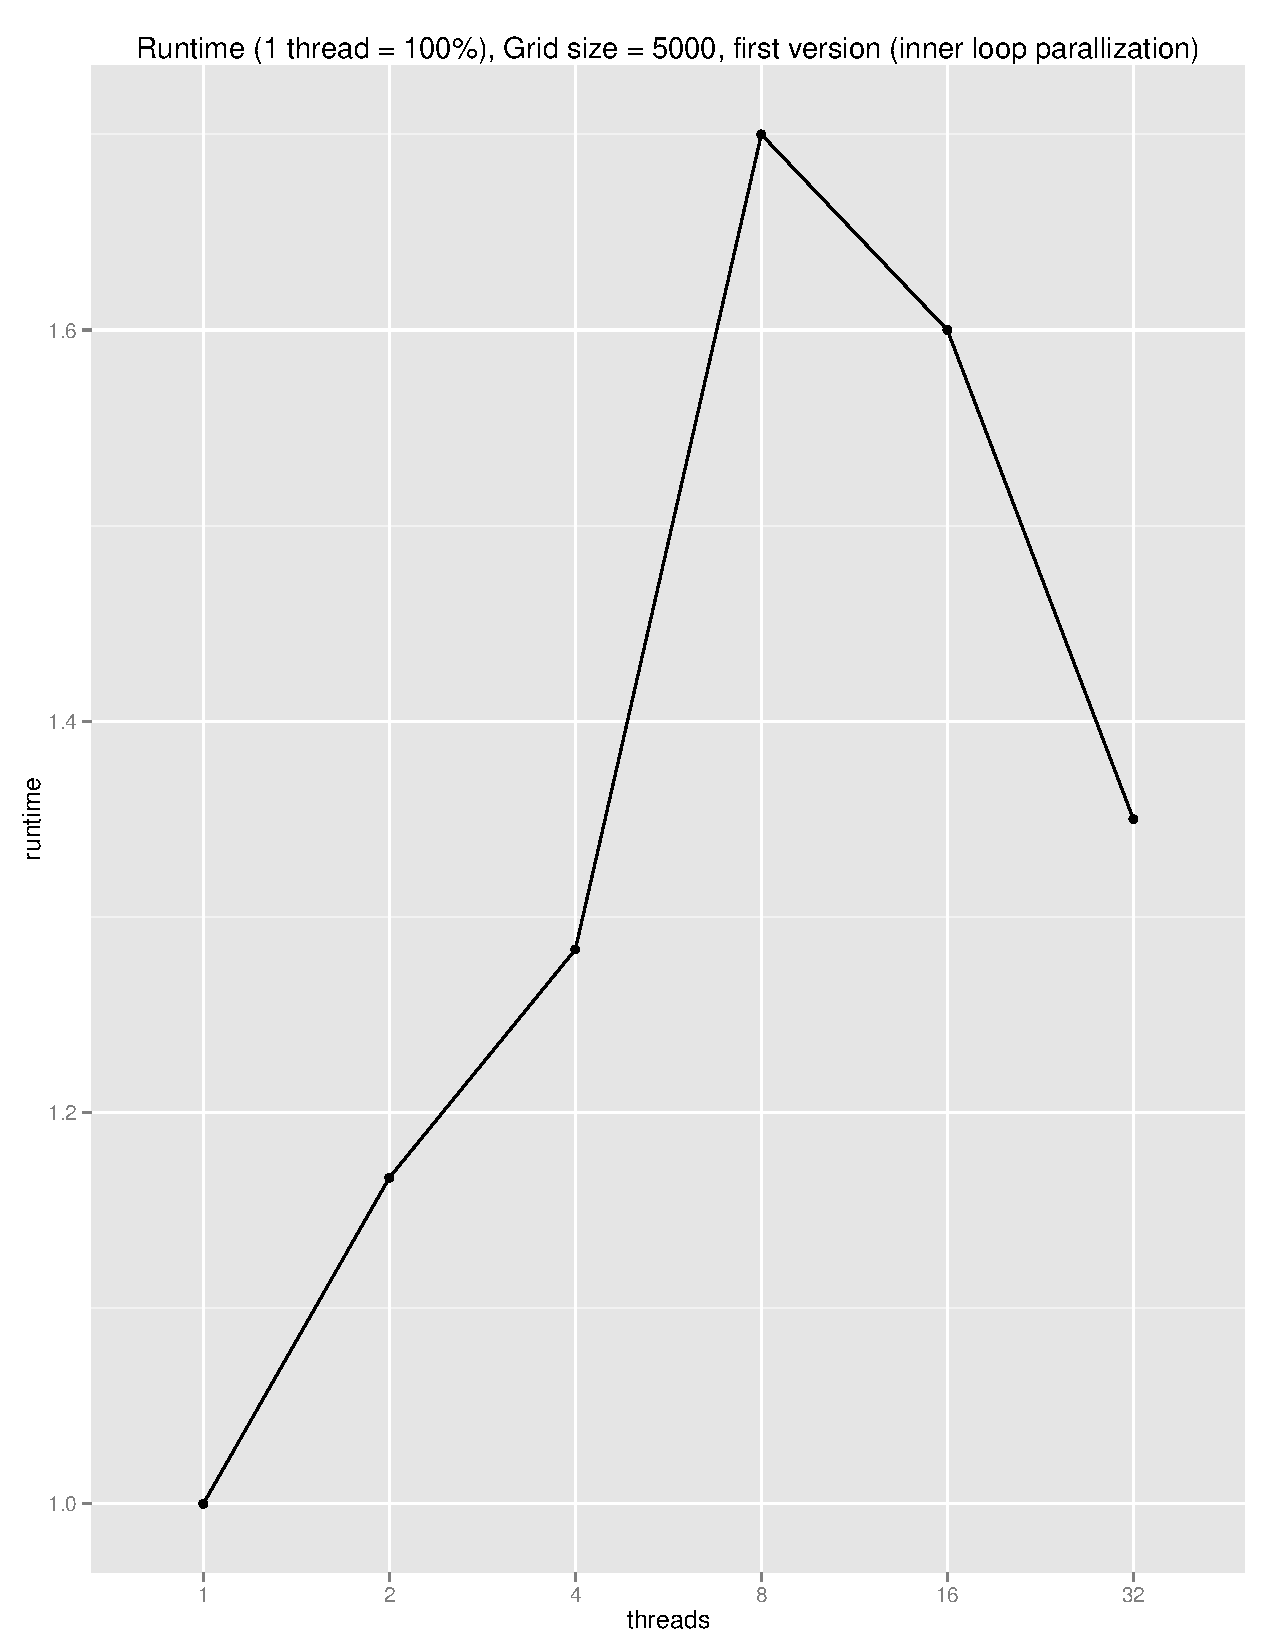
\includegraphics[scale=0.6]{plot1}
%	\caption{Strong (negative) scaling for the attempt of directly parallelizing the inner loop of the serial code, showing a performance that never performed better than the serial version.}
%	\label{fig:plot1}
%\end{figure}


Continuing, we simply parallelized the preceding loop (turning out to be embarrasingly parallel) which displayed a massive speedup. To optimize the speedup, trials with different thread scheduling were performed with the default static sharing proving to work most efficiently, see figure 1. E.g. the dynamic scheduling caused suboptimal behaviour with runtime speedup only appearing at a very high number of threads. Interestingly, a comparison to the theoretical estimation of achievable runtime with increasing number of threads (assuming divided workload with doubled thread number, i.e. $\frac{1}{2^{threads}}$, shows that the outer loop pragma with static scheduling gives a very good performance. Noteworthy is that the small problem size creates a situation where a runtime plateu is never reached with increasing threads (or at least not when being limited to 32 threads). Also, the scaling that is observed (with almost perfect halving of the runtime with a doubled number of threads) is of course also not viewable when approaching extremely small examples (in this case e.g. gridsize $\leq$ 100) for which no improvement can be seen for any parallelization. 

\begin{figure}[]
	\centering
	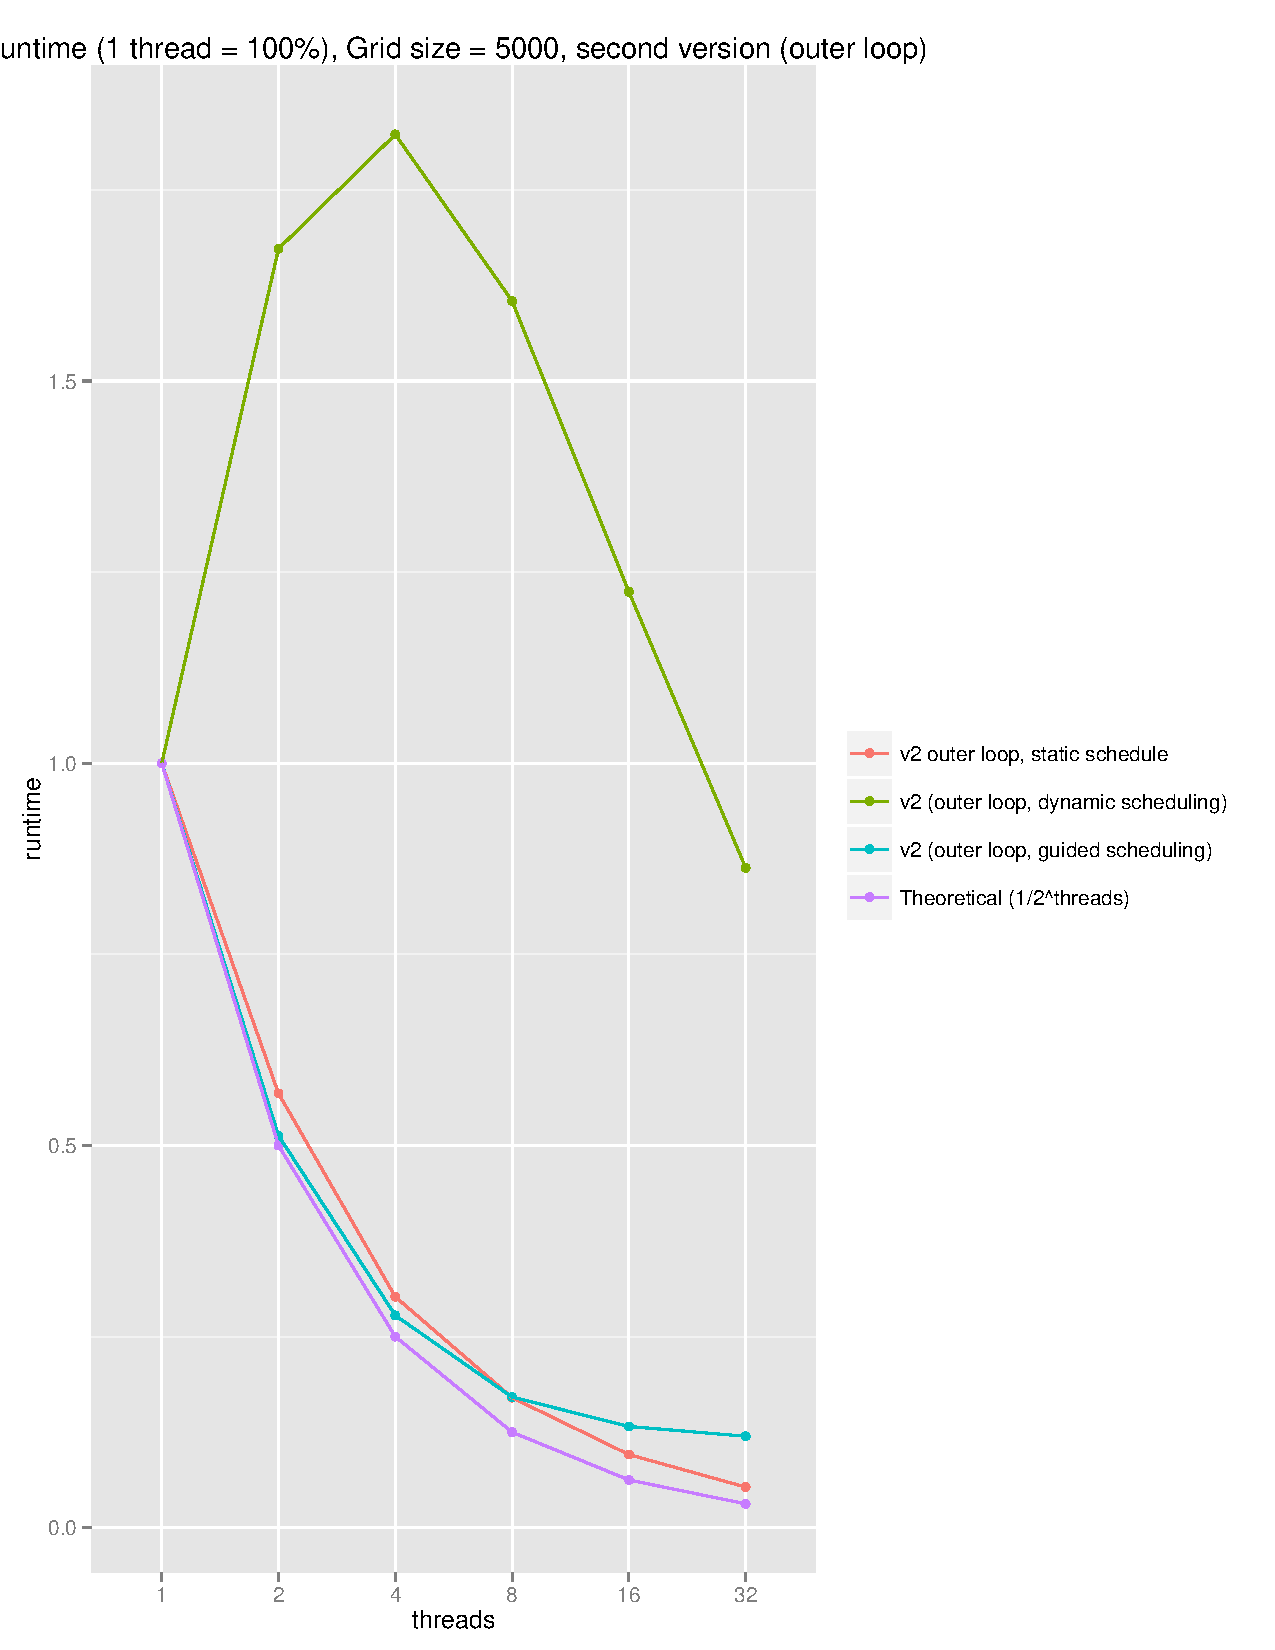
\includegraphics[scale=0.5]{plot2}
	\caption{Strong scaling for the outer loop parallelization of the problem with different scheduling schemes. A simplistic theoretical estimation is added for comparison.}
	\label{fig:plot1}
\end{figure}

Eventhough speedup was acheived for the outer loop pragma, the serial code was modified as to make it simpler to handle following the problems of the inner loop pragma. This included unrolling the for-loop structure entailing only two iterations, as well as combining nested if-statements to a single one. This created a much more clean for-loop structure on which further parallelization schemes could be tested. A code snippet is give below:

\begin{lstlisting}[caption={Restructured for-loops, created for simpler parallelization}, label={lst:L4}]
 for (iteration = 1; iteration <= MAXITER; iteration++)
    {
        memcpy(J_old, J_new, sizeof(*J_new) * DIM);
        {   
            for (int i = 0; i < M; i++)
            {
                for (int e = 0; e < 2; e++)
                { 
                    double c     = (1+r) * k[i] + w*e - kp[0];
                    J_new[e][i]  = sqrt(c) + B*(p0*J_old[0][0]+p1*J_old[1][0]);
                    pol[e][0][i] = k[i];
                    pol[e][1][i] = kp[0];
                    pol[e][2][i] = c;               
                }
                for (int j = 0; j < M; j++)
                {
                    for (int e = 0; e < 2; e++)
                    {
                        double c = (1+r) * k[i] + w*e - kp[j];
                        if ( c >= 0)
                        {
                        double tmp = sqrt(c)+B*( p0*J_old[0][j]+p1*J_old[1][j]);
                          if ( tmp > J_new[e][i] )
                          {
                              J_new[e][i] = tmp;
                              pol[e][0][i] = k[i];
                              pol[e][1][i] = kp[j];
                              pol[e][2][i] = c;
                          }
                        }
                    }
                }
            }
        }
    }
\end{lstlisting}
\section*{Parallelization - second step}
Continuing on with the attempts of parallelizing the code, the nested two-loop structure was deemed sub-optimal in the given situation on Beskow. With the allocated nodes being limited to 32 threads, single threads dividing into multiple threads (potentially possible through \emph{aprun -j}), the idea was to combine the two for-loops doing $N^2$ iterations in one big loop over a single array of indices; a structure that would allow for continuous multithreading. 

To achieve this, iteration arrays for the previous \emph{i} and \emph{j} indices was initialized with entires corresponding to the previous two-loop \emph{i},\emph{j} structure. This generated a single main-loop structure on which multithreading could be performed (note that for some specific indices, certain if-statements where inserted to preserve code output, see upcoming code snippets). However, the same problem with false sharing and potential race conditions which was previously in the inner loop had to be taken into consideration. As seen before though, this approach could potentially lead to suboptimal code behaviour, and instead optimization in code chunking was explored.

OpenMP allows for chunk division by a specific schedule command. Important is that chunks need to be equally sized over all threads. Code-wise this meant divided work equally over all threads. However, being an input of OpenMP, this required that the work could be equally distributed over the threads. For implementation, see code snippet below:

\begin{lstlisting}[caption={Structuring of one for-loop, with OpenMP chunk division}, label={lst:L5}]
int num_threads;
#pragma omp parallel
{
   num_threads = omp_get_num_threads();
}
float divideCheck;
divideCheck = M % num_threads;
if (divideCheck != 0) {
    printf("ERROR: Gridsize %i has to be divisble by the number of threads. %i\n",M,num_threads);
    exit(-1);
}
int thread_num;
int start;
int end;
int chunks;
chunks = M*M/num_threads;
for (iteration = 1; iteration <= MAXITER; iteration++)
{
    memcpy(J_old, J_new, sizeof(*J_new) * DIM);
    #pragma omp parallel for schedule(static,chunks) private(thread_num,num_threads,start,end,j,cnt,c0,c1,c00,t0,c11,t1)
    for (cnt = 0; cnt <arrayLength; cnt++)
    {
     j = cnt % M; 
     if (j==0) {
	     c0 = (1+r) * k[iArray[cnt]] + w*0 - k[0];
         c1 = (1+r) * k[iArray[cnt]] + w*1 - k[0];
         J_new[0][iArray[cnt]] = sqrt(c0) + B*(p0*J_old[0][0] + p1*J_old[1][0]);            
         J_new[1][iArray[cnt]] = sqrt(c1) + B*(p0*J_old[0][0] + p1*J_old[1][0]);
     }
             
     c00 = (1+r) * k[iArray[cnt]] + w*0 - k[j];
     t0 = sqrt(c00) + B * ( p0 * J_old[0][j] + p1 * J_old[1][j] );
     c11 = (1+r) * k[iArray[cnt]] + w*1 - k[j];
     t1 = sqrt(c11) + B * ( p0 * J_old[0][j] + p1 * J_old[1][j] );
 
     if ( c00 >= 0 && t0 >= J_new[0][iArray[cnt]] )
         J_new[0][iArray[cnt]] = t0;
         if ( c11 >= 0 && t1 >= J_new[1][iArray[cnt]] )
             J_new[1][iArray[cnt]] = t1;
         }
    }
\end{lstlisting}

Some important code parts can be highlighted: As said, an error prompt has to be inserted to make sure that equal chunks are provided to the OpenMP (line 8-11). Proceeding, a simple \emph{\color{Plum} \#pragma... schedule(static,chunks)} is inserted on line 21, before the main for-loop. Very important is also the addition of the \emph{\color{Plum} private} variables, such that no false sharing occurs between individual threads. Note also in general the use of the created \emph{iArray} such that the nested two-loop structure could be reduced to a single loop. 

The created chunk-creation using implemented OpenMP \emph{\color{Plum} \#pragma} worked as an elegant parallelization. However, having a code being only able to work on thread numbers equally divisble with the problem size was suboptimal. Therefore, manual chunking was introduced to be able to take care of an arbitrary combination of threads and problem sizes:


\begin{lstlisting}[caption={Manual OpenMP chunk creation}, label={lst:L5}]
int num_threads;
#pragma omp parallel
{
    num_threads = omp_get_num_threads();
}
float divideCheck;
divideCheck = M % num_threads;
int thread_num;
int start;
int end;
 
for (iteration = 1; iteration <= MAXITER; iteration++)
{
	memcpy(J_old, J_new, sizeof(*J_new) * DIM);
    #pragma omp parallel private(thread_num,num_threads,start,end,j,cnt,c0,c1,c00,t0,c11,t1) 
    {
    	thread_num = omp_get_thread_num();
        num_threads = omp_get_num_threads();
        start = thread_num * arrayLength / num_threads;
        end = (thread_num + 1) *arrayLength / num_threads; 
        for (cnt = start; cnt <end; cnt++)
        {
        	j = cnt % M; 
            if (j==0) {
            	c0 = (1+r) * k[iArray[cnt]] + w*0 - k[0];
                c1 = (1+r) * k[iArray[cnt]] + w*1 - k[0];
                J_new[0][iArray[cnt]]    = sqrt(c0) + B * ( p0 * J_old[0][0] + p1*J_old[1][0] );            
                J_new[1][iArray[cnt]]    = sqrt(c1) + B * ( p0 * J_old[0][0] + p1*J_old[1][0] );
			}
                 
            c00 = (1+r) * k[iArray[cnt]] + w*0 - k[j];
            t0 = sqrt(c00) + B * ( p0 * J_old[0][j] + p1 * J_old[1][j] );
            c11 = (1+r) * k[iArray[cnt]] + w*1 - k[j];
            t1 = sqrt(c11) + B * ( p0 * J_old[0][j] + p1 * J_old[1][j] );
     
            if ( c00 >= 0 && t0 >= J_new[0][iArray[cnt]] )
            	J_new[0][iArray[cnt]] = t0;
                if ( c11 >= 0 && t1 >= J_new[1][iArray[cnt]] )
                	J_new[1][iArray[cnt]] = t1;
            }
        }
    }
\end{lstlisting}
At line 17-20, manual chunk sizes are created by relating the specific thread number (through \emph{omp\_get\_num\_threads}) to the start end end index for individual thread iterations. Note that that for the last thread, this will mean proceeding onto the last needed iteration, thus taking care of potential ''mis''matches in thread numbering and problem sizes. 

The run time difference between the manually created chunk threading and implemented OpenMP was in practice identical. Having approched the code in different ways, it is interesting to compare speedup between these different threading approaches. Such information is displayed in Figure 2.

\begin{figure}[]
	\centering
	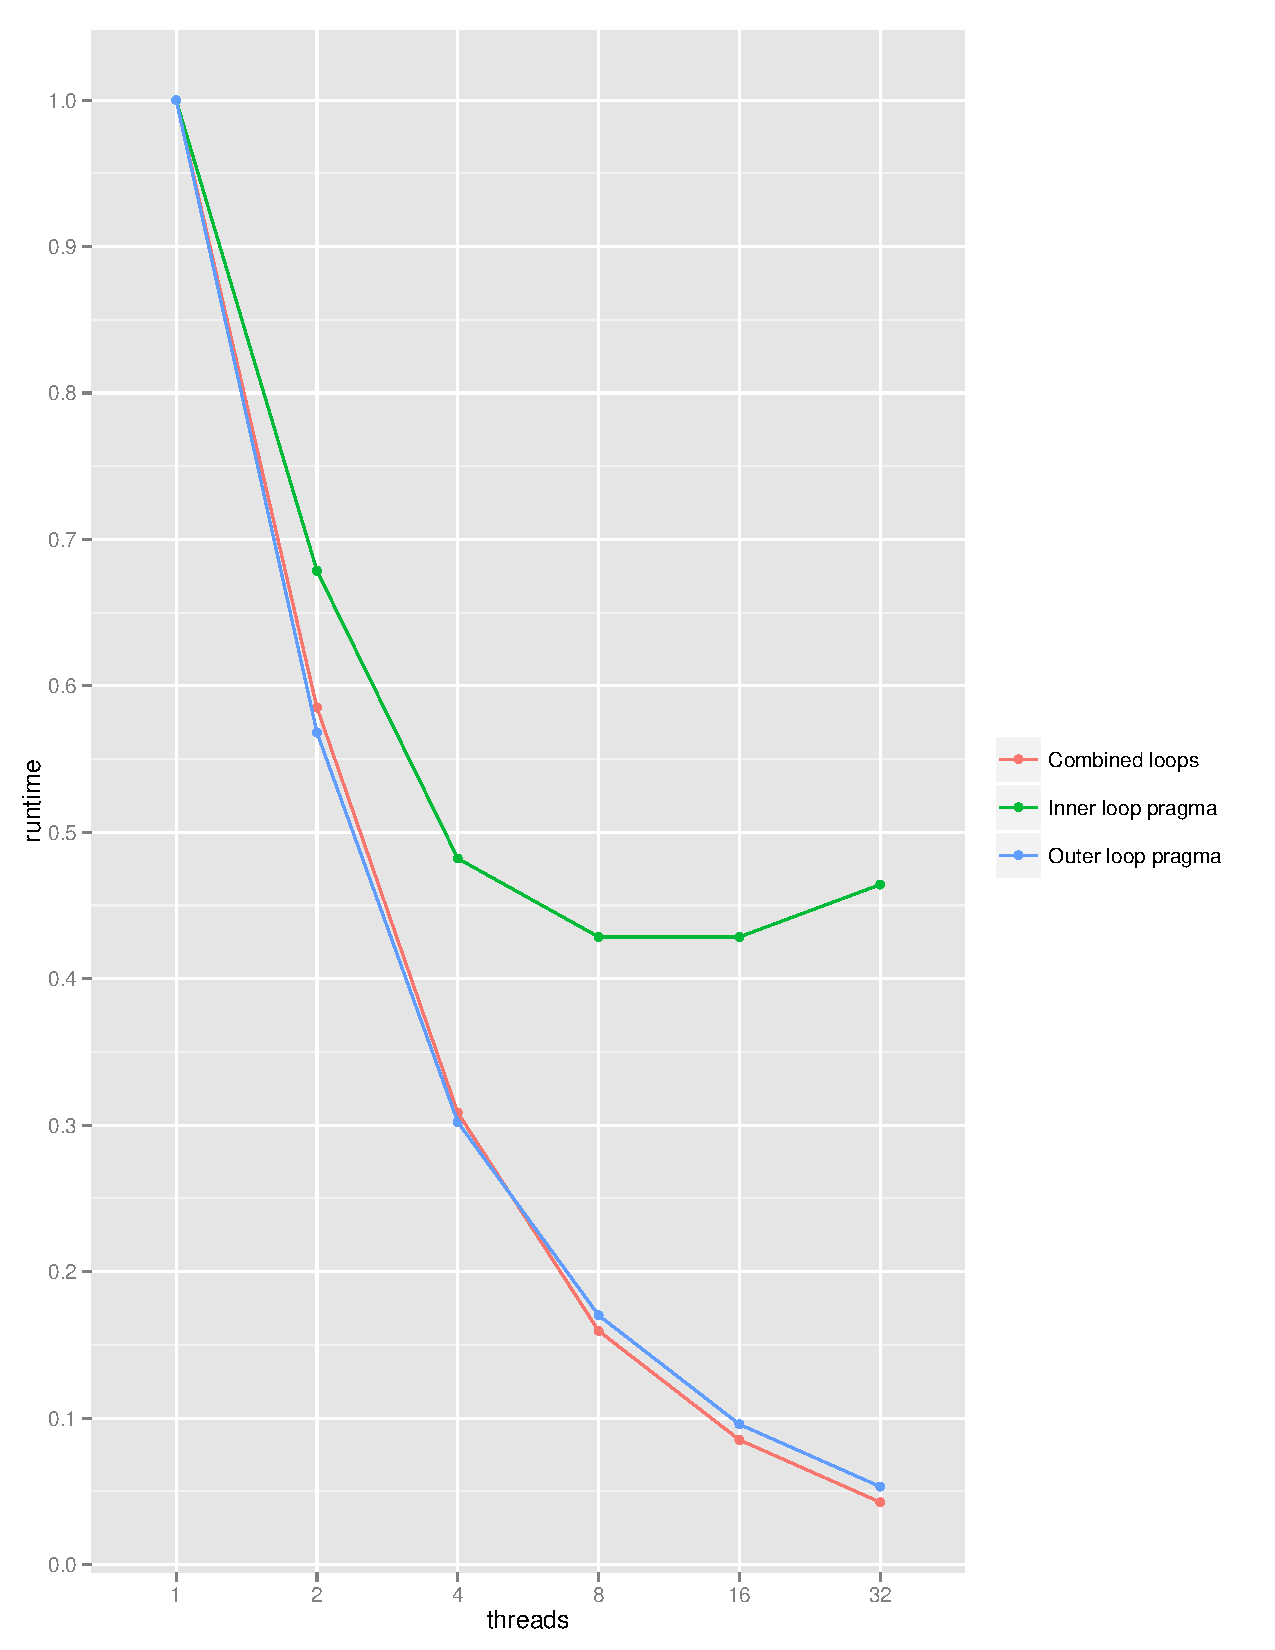
\includegraphics[scale=0.5]{plot3}
	\caption{Strong scaling for multithreading at different parts of the code.}
	\label{fig:plot3}
\end{figure}

As seen, restructuring the serial code fully and creating one main loop (instead of a nested loop-structure) actually gave the optimal speed up (even though differences to the outer loop \emph{\color{Plum} \#pragma} could be regarded as nearly negligible). With the current implementation, going over to a maximum of 32 threads created a significant decrease in run time, requiring a mere 5\% of the initial run time. Interestingly, the inner loop \emph{\color{Plum} \#pragma} where the introduced extra code handling the race condition actually introduces so many new variables and data handling (with multiple variables having to be accessed on and off from cache memory) that such optimization stalled at relatively few threads. With the thread numbers limited to 32, no convergence stalling was seen for the two optimal solutions. In fact, even when scaling up the problem (with an increasing grid size) no general difference was seen and as before, doubling the thread number seem to halve the run time). Interestingly, the problem seem to be so optimal (code wise) that such increasing problem experiments had to be aborted when memory issues on the individual node was encountered (which thus occurred before any potential runtime stalling).  

\begin{figure}[]
	\centering
	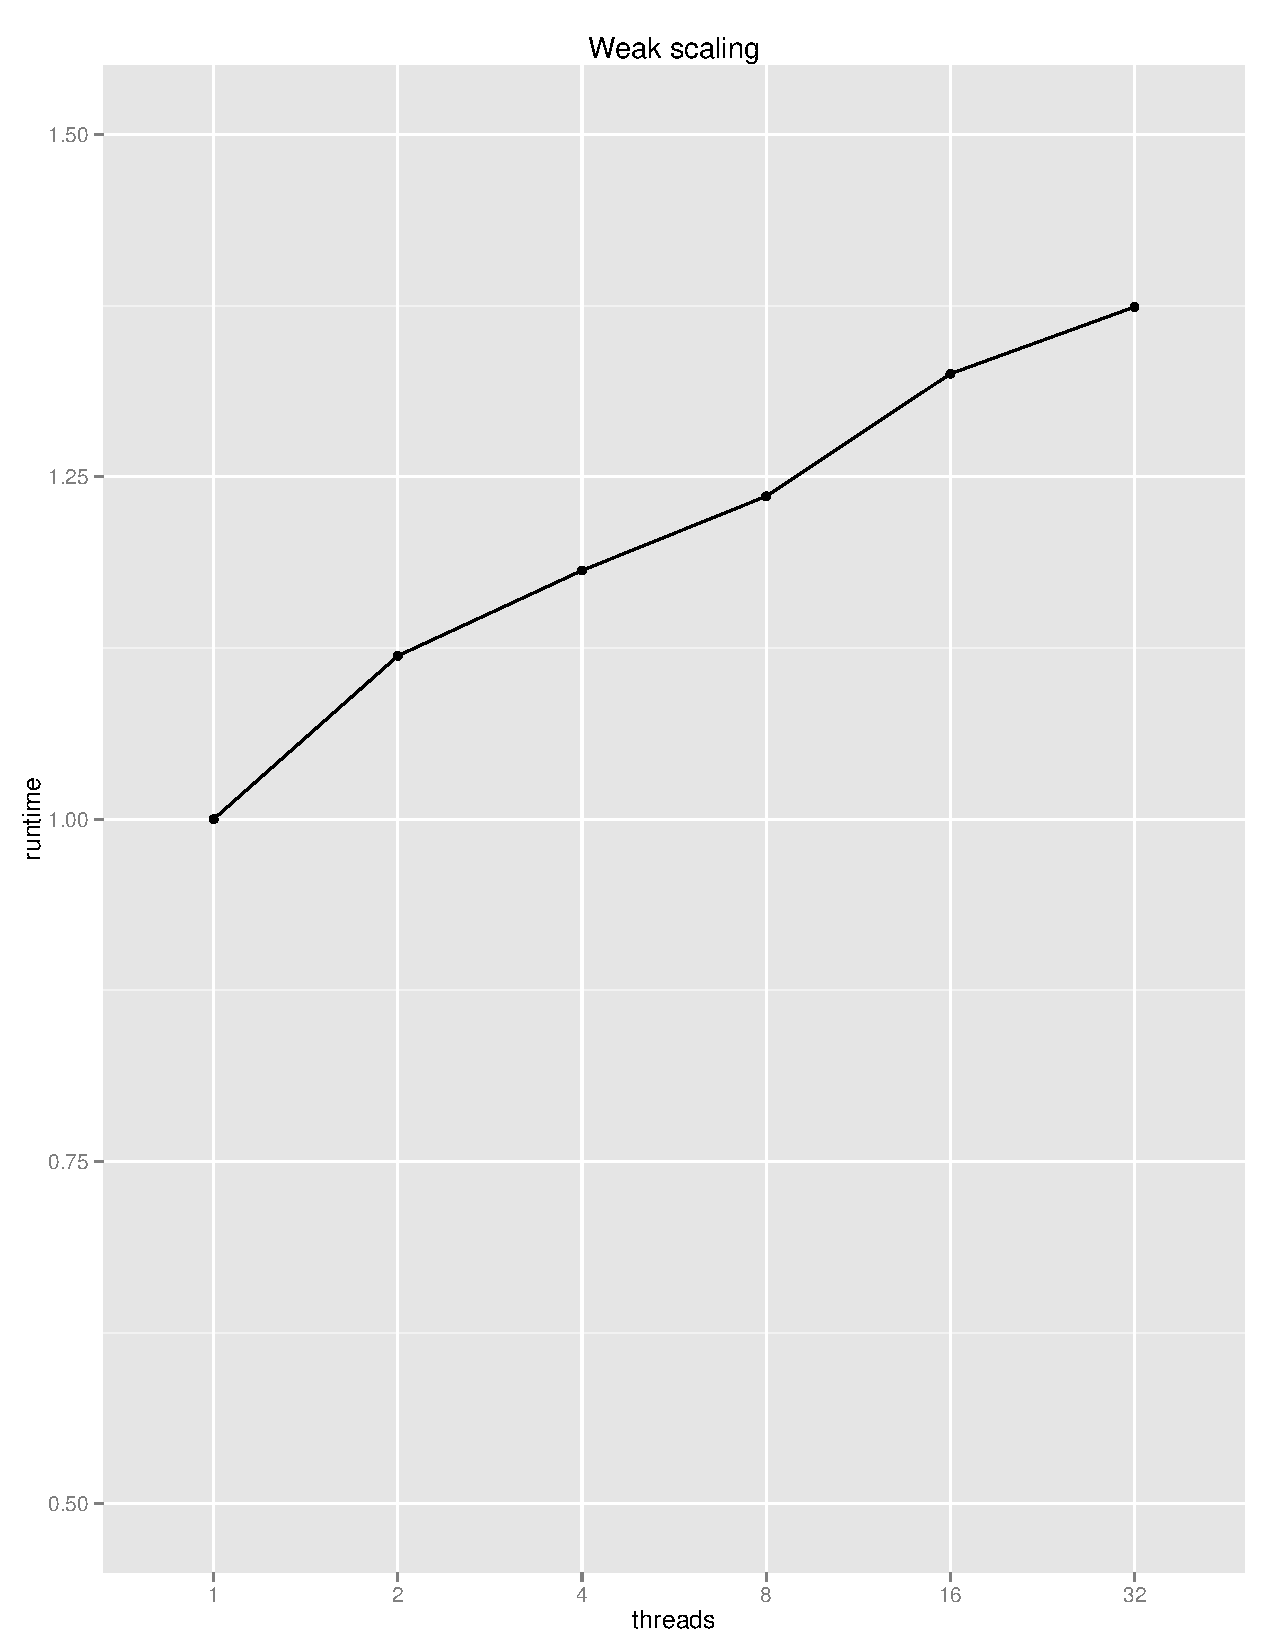
\includegraphics[scale=0.5]{plot4}
	\caption{Weak scaling for the chunk-based multithread implementation.}
	\label{fig:plot3}
\end{figure}

So summarizing the chunk-based \emph{\color{Plum} \#pragma} solution proved optimal when trying a purely OpenMP-based solution to the given problem. Accompanying the strong scaling plot in Figure 2, Figure 3 displays the weak scaling of this particular code. The weak scaling test was achieved by increasing the number of iterations for the same gridsize of the particular tested problem. The weak scaling appears to act as for a generic weak scaling case, with a slight increase in run time with increasing nodes (deviating from the ideal theoretical case of constant run time). 

Judging the code as optimized, a final peformance profiling was performed on the OpenMP code to serve as a comparison to the initial profile report. 

\begin{lstlisting}[caption=CrayPat/X report snippet, label={lst:L6}]
  D1 cache hit,miss ratios          97.2% hits          2.8% misses
  D1 cache utilization (misses)     35.45 refs/miss    4.432 avg hits
  D2 cache hit,miss ratio           98.6% hits          1.4% misses
  D1+D2 cache hit,miss ratio       100.0% hits          0.0% misses
  D1+D2 cache utilization         2624.91 refs/miss  328.114 avg hits
  D2 to D1 bandwidth               44.234MiB/sec   181989568 bytes
\end{lstlisting}

Again, hits for both L1 and L2 are in the high 90's indicating good memory layout and traversing. Interesting is also the comparison to the code line usage:
\begin{lstlisting}[caption=CrayPat/X report snippet, label={lst:L6}]
  Samp% |  Samp | Imb. |  Imb. |Group
        |       | Samp | Samp% | Function
        |       |      |       |  Source
        |       |      |       |   Line
        |       |      |       |    Thread=HIDE
       
 100.0% | 392.0 |   -- |    -- |Total
|----------------------------------------------------------------
|  60.7% | 238.0 |   -- |    -- |ETC
||---------------------------------------------------------------
|  60.2% | 236.0 |   -- |    -- | main
3        |       |      |       |  d/davlars/Lab7/seropenmp_david4.c
||||-------------------------------------------------------------
4|||   2.6% |  10.0 |  5.6 | 58.5% |line.124
4|||  16.3% |  64.0 | 16.2 | 25.3% |line.126
4|||   6.9% |  27.0 | 14.2 | 34.2% |line.134
4|||  11.2% |  44.0 | 38.8 | 35.1% |line.135
4|||   2.0% |   8.0 |  7.9 | 45.2% |line.136
4|||  15.8% |  62.0 | 39.8 | 32.6% |line.137
4|||   3.1% |  12.0 |  9.2 | 26.5% |line.139
4|||   1.5% |   6.0 |  4.7 | 37.0% |line.140
||||=============================================================
||===============================================================
|  38.3% | 150.0 |   -- |    -- |OMP
||---------------------------------------------------------------
|  38.0% | 149.0 |   -- |    -- | _cray$mt_join_barrier
|================================================================
\end{lstlisting}

Again, no big difference to the intial code is seen, even though the work within the inner lines of the general main loop seem to be divided a bit more equally. This correspondence underlines the fact that the simplicity of the used code, in the sense that one optimization task was performed at one specific case. As shown by the OMP-memory usage, the main work seems though to be entailed within the multithreading of the program, indicating a successful parallelization of the code. 

As a final discussion, an MPI approach to the given problem was initially investigated where, in the case of a preserved two-loop structure, the outer loop could be MPI-split over several nodes whereafter some multithread OpenMP approach could proceed on each node. However, the layout of the program was considered suboptimal for an MPI approach. The program consists of a series of two-dimensional arrays allocated as one contiguous piece of storage. This could be potentially split over several processors but would need a lot of manual data handling and passing of information after each loop update. Even more complex, the main array used in the optimization is a three-dimensional array for which MPI-handling would become quite cumbersome (forcing the program to allocate pointers to pointers to pointers). Judging from the program size and complexity, this was deemed non-efficient in comparison to a full OpenMP-approach.

 \section*{Summary}
In this project we attempted to parallelize a serial C program doing value function iteration. We discovered how hard concurrency was, and learned the value of looking for the easiest (most embarrassingly parallel part) to work on first. In our case this led to a huge speedup (perfectly utilizing all 32 cores on a Beskow node. 

As for user friendliness, we appreciated the power of OpenMP's simple pragmas. In comparison, MPI is much more low-level, and brings us closer to implementation than problem solving (of course our problem was not really of a sufficient size to be suitable for a multinode MPI solution).

For our future work we have gotten a valuable insight into HPC. Even though we are probably not going to immediately head out and  book a 100 node job on Beskow, our knowledge of OpenMP could be put to use on our personal multicore computer (with a suitable compiler, GCC for example).



\newpage
\section*{Appendix A}
\subsection*{Original serial code (directly translated from Python)}

\begin{lstlisting}[caption=Original serial code, label={lst:LAppendix}]
#include<stdio.h>
#include<stdlib.h>
#include<string.h>
#include<math.h>
 
const double THRESH = 1E-6;
const int DIM       = 2;
const int DEP       = 3;
const double B      = 0.95;
const double r      = 0.04;         
const double w      = 1.0;  
const double p0     = 0.1;  
const double p1     = 0.9;
const double A      = 50.0; // Artifical problem size
 
int M;
int MAXITER;
int iteration;
 
int converged(double (*parr1)[M], double (*parr2)[M], double (*pdiff)[M], const int size)
{
    double maxd1 = 0, maxd2 = 0;
 
    for (int i = 0; i < size; i++)
    {
        pdiff[0][i] = fabs (parr1[0][i] - parr2[0][i]);
        pdiff[1][i] = fabs (parr1[1][i] - parr2[1][i]);
        if ( pdiff[0][i] > maxd1 )
            maxd1 = pdiff[0][i];
        if ( pdiff[1][i] > maxd2 )
            maxd2 = pdiff[1][i];
    }
    return ((maxd1 < THRESH) && (maxd2 < THRESH)) ? 1 : 0; 
}
 
void printres(double (*parr)[M], double** ppol[], const int size)
{
    printf("J[0]\tk[0]\tkp[0]\tc[0]\tJ[1]\tk[1]\tkp[1]\tc[1]\n");
    for (int i = 0; i < size; i++)
        printf("%.3f\t%.3f\t%.3f\t%.3f\t%.3f\t%.3f\t%.3f\t%.3f\n",
         parr[0][i], ppol[0][0][i], ppol[0][1][i], ppol[0][2][i], 
         parr[1][i], ppol[1][0][i], ppol[1][1][i], ppol[1][2][i]);
}
 
 
int main(int argc, char** argv)
{
    if (argc == 1) 
    {
        printf("Usage: \n");
        printf("%s GridSize MaxIter\n", argv[0]);
        return 0;
    }
     
    M  = atoi (argv[1]);
    MAXITER  = atoi (argv[2]);
 
    double** pol[DIM];
    for (int i = 0; i < DIM; i++)
    {
        pol[i]   = (double **) malloc(DEP * sizeof(double));
        for (int j = 0; j < DEP; j++)
            pol[i][j] = (double *) malloc(M * sizeof(double));
    }
 
    double *k  = calloc(M, sizeof(double));
    double *kp = calloc(M, sizeof(double));
    for (int i = 1; i < M; i++)
        k[i] = kp[i] = k[i-1] + A / (M-1);  // Initialize grid
     
    // Alt. malloc: double (*arr)[COLS] = malloc( ROWS * sizeof *arr)
    double (*J_new)[M] = malloc(sizeof (*J_new) * DIM);
    double (*J_old)[M] = malloc(sizeof (*J_old) * DIM);
    double (*diff)[M]  = malloc(sizeof (*diff) * DIM);
 
    for (int i = 0; i<DIM; i++)
    {
        for (int j=0; j<M; j++)
        {
            J_new[i][j] = J_old[i][j] = 0;
        }
    }
 
    for (iteration = 1; iteration <= MAXITER; iteration++)
    {
        memcpy(J_old, J_new, sizeof(*J_new) * DIM);
        for (int i = 0; i < M; i++)
        {
            for (int e = 0; e < 2; e++)
            {
                double c     = (1+r) * k[i] + w*e - kp[0];
                J_new[e][i]  = sqrt(c) + B * ( p0 * J_old[0][0]+p1*J_old[1][0]);
                pol[e][0][i] = k[i];
                pol[e][1][i] = kp[0];
                pol[e][2][i] = c;               
            }
            for (int j = 0; j < M; j++)
            {
                for (int e = 0; e < 2; e++)
                {
                    double c = (1+r) * k[i] + w*e - kp[j];
                    if ( c >= 0)
                    {
                    double tmp = sqrt(c) + B*(p0*J_old[0][j]+p1*J_old[1][j]);
                        if ( tmp > J_new[e][i] )
                        {
                            J_new[e][i] = tmp;
                            pol[e][0][i] = k[i];
                            pol[e][1][i] = kp[j];
                            pol[e][2][i] = c;
                        }
                    }
                }
            }
        }
    }
    if ( converged(J_old, J_new, diff, M) ) 
        {
            printres(J_new, pol, M);
            return 0;
        }
    else
        printf("Did not converge\n");
 
}
\end{lstlisting}




























\end{document}